\documentclass[11pt]{article}
\usepackage[utf8]{inputenc}
\usepackage[T1]{fontenc}
\usepackage{hyperref}
\hypersetup{colorlinks=true, linkcolor=blue, filecolor=magenta, urlcolor=cyan,}
\urlstyle{same}
\usepackage{amsmath}
\usepackage{amsfonts}
\usepackage{amssymb}
\usepackage{booktabs}
\usepackage{geometry}
\usepackage{palatino}
\geometry{a4paper, margin=3cm}

\usepackage{graphicx}
\usepackage[export]{adjustbox}
\graphicspath{ {./images/} }
\usepackage{caption}
\usepackage{subcaption}
\usepackage{listings}
\usepackage{xcolor}

\lstdefinestyle{mypython}{
  language=Python,
  basicstyle=\ttfamily\footnotesize,
  keywordstyle=\color{blue}\bfseries,
  stringstyle=\color{red!70!black},
  commentstyle=\color{gray}\ttfamily\itshape,
  showstringspaces=false,
  breaklines=true,
  backgroundcolor=\color{gray!5},
  frame=single,
  rulecolor=\color{gray!30}
}

\lstset{style=mypython}

\title{\textbf{ELEC0447 -- Project 2} \\[2mm] 
\Large Transmission System Steady-State Modeling, \\Security, and Energy Transition Analysis}
\author{Prof. Bertrand Corn\'elusse}
\date{November 12, 2026 -- Version 1.0}

\begin{document}
\maketitle

\section{Introduction and Objectives}
The objective of this assignment is to deepen your understanding of modern transmission system analysis, operation, and grid planning using the open-source Python library PandaPower. Refer to the \href{https://pandapower.readthedocs.io/en/}{documentation of PandaPower} for more information.

This project explores real-world challenges encountered by transmission system operators in the context of the energy transition, such as
steady-state power flow and voltage/reactive power management ($P$-$V$ curves, shunt compensation), 
primary frequency control and distributed slack power flow modeling, 
short-circuit current calculations and grid strength / rotor angle stability assessment, time-varying renewable generation dynamics (solar PV, wind, and demand duck curve), grid expansion and reinforcement, and $N-1$ security under massive load growth and remote renewable integration.


\subsection{Benchmark: The IEEE 24-Bus Reliability Test System}
We consider a standard, publicly available transmission grid benchmark: the \textbf{IEEE 24-Bus Reliability Test System (RTS)}. It has two voltage levels: 
a northern $230\text{ kV}$ extra-high-voltage (EHV) network (Buses 11--24) and a southern $138\text{ kV}$ high-voltage (HV) network (Buses 1--10).
5 transformers connect the $230\text{ kV}$ northern backbone to the $138\text{ kV}$ southern subtransmission grid.
The northern area is rich in generation (hydro, nuclear, large thermal units, and vast renewable potential), whereas the southern area represents a dense, heavily loaded industrial and urban pocket.

%TOD improve geo plot, put a diagram from the net.
\begin{figure}[h!]
  \centering
  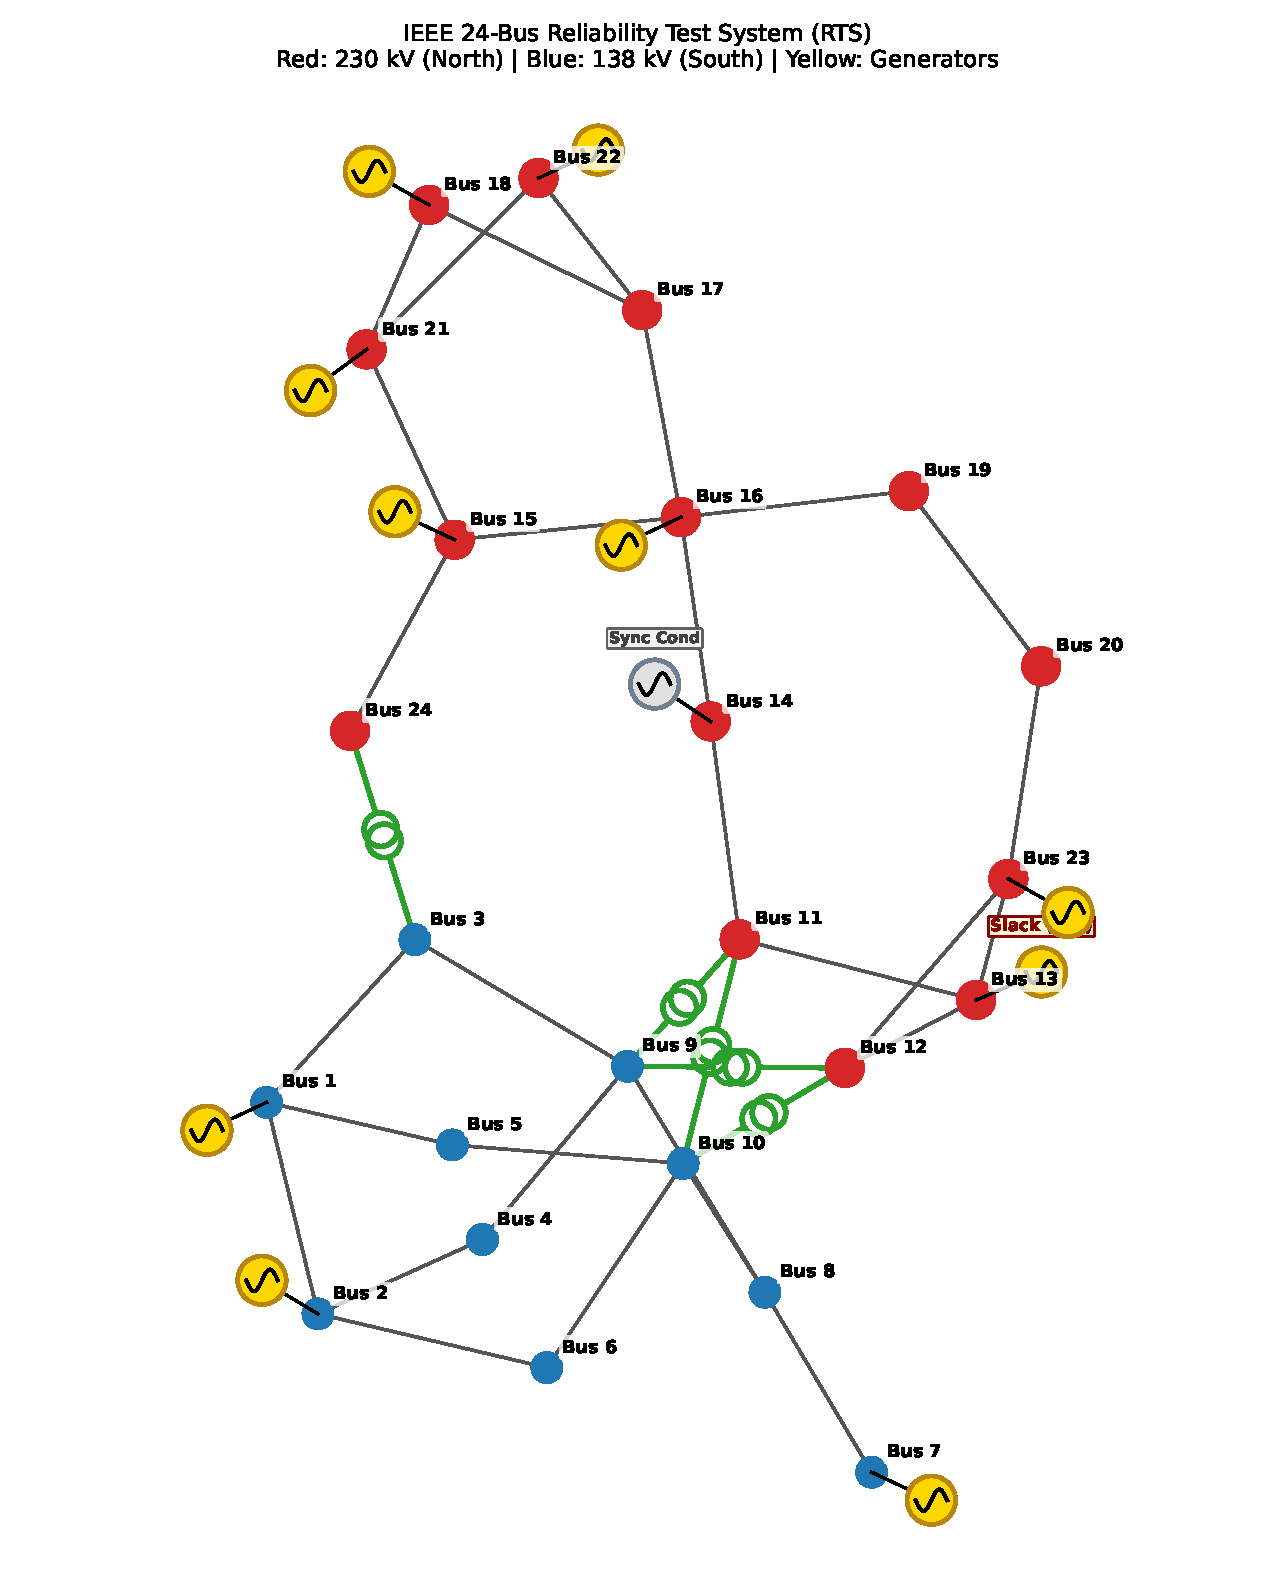
\includegraphics[width=\textwidth]{rts24_map.pdf}
  \caption{Geographical layout (North: 230 kV, South: 138 kV) with highlighted generation units and slack bus.}
  \label{fig:rts24_map}
\end{figure}

% or via the provided file \lstinline|Pandapower_ieee24_rts.json| on eCampus:
\begin{lstlisting}[language=Python, caption=The network can be loaded directly from PandaPower.]
import pandapower as pp
import pandapower.networks as nw
net = nw.case24_ieee_rts()
\end{lstlisting}
%# Option B: From the enriched project JSON file (with preconfigured SC and droop parameters)
%net = pp.from_json("Pandapower_ieee24_rts.json")

\clearpage


%\section{Technical Primer: Concepts Beyond the Standard Lecture Slides}
%To complete this assignment successfully, you will need two key modeling concepts that bridge steady-state power flow and power system dynamics.
%
%\subsection{Distributed Slack Power Flow and Governor Droop Response}
%In standard Newton-Raphson power flow, a single \textbf{slack bus} balances total system active power:
%\begin{equation}
%  P_{\text{slack}} = \sum_{j} P_{\text{load}, j} + P_{\text{losses}} - \sum_{i \neq \text{slack}} P_{\text{gen}, i}
%\end{equation}
%While computationally convenient, having a single bus absorb all disturbances is physically unrealistic. 
%
%During the \textbf{primary frequency control} timeframe (first $2\text{--}30\text{ seconds}$), all synchronous generators equipped with speed governors react to a frequency deviation $\Delta f$ according to their \textbf{droop} (or statism) $\sigma_i$:
%\begin{equation}
%  \Delta P_i = - \frac{P_{N,i}}{\sigma_i} \cdot \frac{\Delta f}{f_N} = - K_{p,i} \cdot \frac{\Delta f}{f_N}
%\end{equation}
%Summing over all generators and accounting for system damping $D$ gives the quasi-steady-state frequency deviation following an active power imbalance $\Delta P_{\text{imb}}$:
%\begin{equation}
%  \Delta f = - \frac{\Delta P_{\text{imb}} + \Delta P_{\text{losses}}}{\sum_{i} K_{p,i} + D}
%\end{equation}
%Each generator therefore contributes a fraction of the imbalance proportional to its participation factor:
%\begin{equation}
%  w_i = \frac{K_{p,i}}{\sum_{j} K_{p,j}} = \frac{P_{N,i} / \sigma_i}{\sum_{j} (P_{N,j} / \sigma_j)}
%\end{equation}
%In PandaPower, setting \lstinline|distributed_slack=True| and assigning \lstinline|slack_weight| directly mimics this primary frequency response!
%
%\subsection{Short-Circuit Capacity, Grid Strength, and Rotor Angle Stability}
%As established in our \textit{Transient Stability} lecture, a substation bus's short-circuit current reflects the underlying Thévenin driving-point impedance of the interconnected grid ($I''_k \approx \frac{c \cdot V_n}{\sqrt{3} X_{th}}$, $S''_{sc} \approx \frac{c \cdot V_n^2}{X_{th}}$), evaluated immediately post-fault ($t \approx 10\text{--}40\text{ ms}$) where synchronous machines feed large subtransient currents ($5\text{ to }7 \times I_n$) behind $X''_d$.
%
%In addition to sizing switchgear breaking ratings according to the \textbf{IEC 60909} standard, short-circuit power directly governs \textbf{rotor angle stability}:
%\begin{itemize}
%  \item \textbf{Transient Stability \& Equal Area Criterion}: The electrical power delivered by a synchronous generator to the grid is bounded by $P_{\max} = \frac{E' V}{X'_d + X_{th}}$. A high short-circuit level ($X_{th}$ small) expands the post-fault power transfer capability, vastly enlarging the \textbf{decelerating area (Area B)}, increasing the critical clearing angle $\delta_{cct}$, and lengthening the \textbf{Critical Clearing Time ($CCT$)}.
%  \item \textbf{Small-Signal Synchronizing Torque}: A stronger grid directly boosts the synchronizing torque coefficient $K_s = \left.\frac{\partial P_e}{\partial\delta}\right|_{\delta_0} = \frac{E' V}{X'_d + X_{th}} \cos\delta_0$, stiffening electromechanical coupling and preventing aperiodic rotor drift.
%\end{itemize}
%
%The \textbf{Short-Circuit Ratio (SCR)} measures this electrical stiffness relative to the rating of converter-interfaced renewable energy sources (RES):
%\begin{equation}
%  \text{SCR}_i = \frac{S''_{sc,i}}{P_{\text{RES, rated}}}
%\end{equation}
%where $\text{SCR} > 3.0$ denotes a strong grid, $2.0 \le \text{SCR} \le 3.0$ indicates a weak grid with elevated sensitivity to power swings, and $\text{SCR} < 2.0$ identifies very weak grids where standard phase-locked loops (PLLs) can lose synchronism.
%
\clearpage

\section{Questions}

\textbf{Unless explicitly stated, each question below must be solved independently, starting from the baseline grid.} 
Include clear, interpretable, and properly formatted plots. Ensure that every graph supports your technical discussion.

\subsection{Baseline AC Power Flow and Operating Envelope}
  \noindent\textit{\textbf{Course References:} \href{https://github.com/bcornelusse/ELEC0447-analysis-power-systems/blob/master/Lectures/IntroPowerFlow/main.pdf}{Lecture: Introduction to Power Flow Analysis} (AC Newton-Raphson, bus types, DC power flow) and \href{https://github.com/bcornelusse/ELEC0447-analysis-power-systems/blob/master/Lectures/SynchronousGenerator/main.pdf}{Lecture: Synchronous Generators} (generator reactive limits $Q_{\min}/Q_{\max}$).}
  \begin{itemize}
    \item Run an AC Newton-Raphson power flow on the initial grid with generator reactive power limits enforced (\lstinline|enforce_q_lims=True|).
    \item Display the voltage profile and branch loadings using matplotlib.
    \item Include an interactive plot of the network generated with Plotly (\lstinline|pf_res_plotly|). Ensure the substation voltages and line loadings are clearly displayed, and that the \textbf{slack bus} (connected to the external grid reference) is highlighted.
    \item Are all substation voltages within standard statutory limits $[0.95, 1.05]\text{ pu}$? 
    \item Which corridors or transformers are heavily loaded ($>80\%$ of thermal capacity)?
    \item Run a DC power flow (\lstinline|pp.rundcpp(net)|) and compare total transmission losses and branch flows with the AC results. Why are reactive power flows and voltage drops significant in EHV transmission?
  \end{itemize}

  \subsection{Primary Frequency Response and Distributed Slack Power Flow}
  \noindent\textit{\textbf{Course References:} \href{https://github.com/bcornelusse/ELEC0447-analysis-power-systems/blob/master/Lectures/frequency_control/main.pdf}{Lecture: Frequency Control} (governor droop $\sigma$, multi-generator primary power sharing, and analytical frequency deviation $\Delta f$).}
  \begin{itemize}
    \item Simulate the sudden loss (tripping) of the generating unit connected at Bus 23 ($P_{\text{lost}} = 155\text{ MW}$).
    \item \textbf{Single Slack Case}: Run the power flow using the default single slack bus. Observe the resulting generation redispatch and line loadings.
    \item \textbf{Distributed Slack Case}: Assuming all remaining units have a governor droop of $\sigma = 4\%$ ($0.04$), assign \lstinline|slack_weight = sn_mva / droop| to each generator and re-run with \lstinline|pp.runpp(net, distributed_slack=True)|.
    \item Compare the active power output adjustments ($\Delta P_i$) of the generators and the loading of the transmission lines between single slack and distributed slack.
    \item Using the analytical formula from the course, calculate the expected quasi-steady-state frequency deviation $\Delta f$ (assuming $f_N = 50\text{ Hz}$ and damping $D \approx 0$).
  \end{itemize}
  \textcolor{red}{For all subsequent steady-state power flow analyses (Question 3 onward), retain the distributed slack configuration (\lstinline|distributed_slack=True|) so that power flow redispatch realistically reflects governor-droop sharing across the generator fleet.}

  \subsection{Voltage Stability, $P$-$V$ Nose Curves, and Shunt Compensation}
  \label{sec:voltage_stability}
  \noindent\textit{\textbf{Course References:} \href{https://github.com/bcornelusse/ELEC0447-analysis-power-systems/blob/master/Lectures/voltage_stability/voltage_stability.pdf}{Lecture: Voltage Regulation and Voltage Instability} (maximum power transfer, $P$-$V$ nose curves, saddle-node bifurcation, generator reactive limits, and shunt compensation).}
  \begin{itemize}
    \item Disconnect the synchronous generator at Bus 1 and progressively ramp up the active power consumption of the load at Bus 3, maintaining a constant power factor.
    \item Plot the bus voltage magnitude as a function of the consumed active power ($P$-$V$ curve) until the power flow diverges (why does it diverge?).
    \item Compare the $P$-$V$ curves for:
    \begin{enumerate}
      \item Enforcing generator reactive power limits vs. neglecting them.
      \item Two power factor values: $\cos \phi = 1.0$ and $\cos \phi = 0.95$ lagging.
    \end{enumerate}
    \item Determine the maximum permissible power transfer ($P_{\text{max}}$) and the voltage stability margin.
    \item The TSO wants to install a $100\text{ MVAR}$ shunt capacitor bank to improve the voltage profile and push back the collapse point. Test placing it at Bus 3 versus Bus 9. Motivate your choice with simulations.
  \end{itemize}

  \subsection{Subtransient Short-Circuit Current Computation, Grid Strength, and Rotor Angle Stability}
  \noindent\textit{\textbf{Course References:} \href{https://github.com/bcornelusse/ELEC0447-analysis-power-systems/blob/master/Lectures/transient/main.pdf}{Lecture: Transient Stability} (subtransient reactance $X''_d$, IEC 60909 short circuits, Equal Area Criterion, $CCT$, synchronizing torque $K_s$, and Short-Circuit Ratio $SCR$) and \href{https://github.com/bcornelusse/ELEC0447-analysis-power-systems/blob/master/Lectures/intro_stability/intro_stability.pdf}{Lecture: Introduction to Stability and Control Problems}.}
  \begin{itemize}
    \item Configure the generator subtransient parameters ($X''_d = 0.20\text{ pu}$, $R_s = 0.05\text{ }\Omega$, $\cos \phi = 0.85$) and external grid short-circuit level ($S''_{sc} = 5\,000\text{ MVA}$, $R/X = 0.1$).
    \item Run an IEC 60909 three-phase short-circuit calculation using \lstinline|pandapower.shortcircuit.calc_sc(net, fault='3ph', case='max')|.
    \item Plot the initial symmetrical short-circuit current $I''_k\text{ [kA]}$ and short-circuit power $S''_{sc}\text{ [MVA]}$ across all 24 buses.
    \item Compare the northern $230\text{ kV}$ area with the southern $138\text{ kV}$ area. Which bus is electrically the \textit{strongest}? Which is the \textit{weakest}? 
    \item \textbf{Link with Rotor Angle Stability}: Drawing upon the Equal Area Criterion and swing equations from the lectures:
    \begin{enumerate}
      \item How does the local short-circuit power $S''_{sc}$ (and Thévenin reactance $X_{th}$) influence the peak electrical power $P_{\max}$, the decelerating area (Area B), and the Critical Clearing Time ($CCT$) of a synchronous generator following a three-phase fault?
      \item How does a strong grid ($X_{th}$ small) affect the small-signal synchronizing torque coefficient $K_s$ and the spatial spread of fault-induced voltage dips?
    \end{enumerate}
    \item Suppose a developer plans to connect a $500\text{ MW}$ offshore wind farm. Evaluate the Short-Circuit Ratio (SCR) if connected to Bus 3 versus Bus 15. What are the operational implications for grid strength and stability?
  \end{itemize}

  \subsection{Time-Varying Data and Renewable Generation Variability}
  \noindent\textit{\textbf{Course References:} \href{https://github.com/bcornelusse/ELEC0447-analysis-power-systems/blob/master/Lectures/intro_stability/intro_stability.pdf}{Lecture: Introduction to Stability and Control Problems} (net load variations, Duck curve phenomenon) and \href{https://github.com/bcornelusse/ELEC0447-analysis-power-systems/blob/master/Lectures/voltage_stability/voltage_stability.pdf}{Lecture: Voltage Regulation} (impact of RES on grid operating envelope).}
  \vspace{1mm}
  \begin{itemize}
    \item Consider the 24-hour normalized profiles for system demand, solar PV generation, and wind power generation provided in \lstinline|profiles_24h.csv| on eCampus.
    \item To reflect day-ahead operational planning, the dataset also includes a pre-scheduled conventional generation production plan (\lstinline|conv_dispatch_factor|), balancing expected net demand ($D - P_{\text{solar}} - P_{\text{wind}}$), along with technology breakdowns (hydro, nuclear, coal, gas).
    \item Equip the network with $500\text{ MW}$ of solar PV in the south ($250\text{ MW}$ each at Bus 3 and Bus 5) and $250\text{ MW}$ of wind in the north (Bus 19).
    \item For each hour $h \in \{0, \dots, 23\}$, update system active and reactive loads, set renewable generation, scale conventional active setpoints with \lstinline|conv_dispatch_factor|, and run the power flow with distributed slack enabled (\lstinline|distributed_slack=True, enforce_q_lims=True|).
    \item Plot the daily trajectory of:
    \begin{enumerate}
      \item Total system active power demand, solar, wind, and conventional dispatch (stacked area or lines).
      \item The maximum transmission line loading percentage over time.
      \item Minimum and maximum substation voltages over the 24 hours.
    \end{enumerate}
    \item At which hour is the transmission network under the greatest thermal stress? At which hour do we observe the lowest voltage?
    \item Discuss the "duck curve" phenomenon: how does midday solar PV relieve transmission loading and fuel consumption, and why does the sudden loss of solar generation at dusk combined with peak demand create severe ramping and reactive power / voltage challenges?
  \end{itemize}

  \subsection{Grid Expansion: Massive Load Growth, Remote Renewable Boom, and $N-0$ Reinforcements}
  \label{sec:grid_expansion}
  \noindent\textit{\textbf{Course References:} \href{https://github.com/bcornelusse/ELEC0447-analysis-power-systems/blob/master/Lectures/HVDC/main.pdf}{Lecture: High Voltage DC Transmission} (VSC-HVDC operating principles, four-quadrant control, and power flow modeling with \lstinline|pp.create_dcline|) and \href{https://github.com/bcornelusse/ELEC0447-analysis-power-systems/blob/master/Lectures/TransfomerAndPF/main.pdf}{Lecture: Transformers} (Phase-Shifting Transformers).}
  \vspace{1mm}
  \begin{itemize}
    \item To reflect the decarbonization of industry and heating, the active and reactive demand in the southern region (Buses 1--10) increases permanently by \textbf{$+40\%$}.
    \item In parallel, $1\,500\text{ MW}$ of fossil-fired generation in the south is decommissioned, replaced by $2\,500\text{ MVA}$ of remote wind generation connected at the northern extremity (Bus 22), injecting $1\,500\text{ MW}$ under high-wind conditions.
    \item Simulate the intact system ($N-0$ state):
    \begin{itemize}
      \item Which transmission corridors connecting the north to the south are severely overloaded ($>100\%$)? How is the bus voltage profile impacted across the 138~kV and 230~kV subsystems?
      \item How does the decommissioning of southern synchronous machines affect the short-circuit level ($S''_{sc}$) and grid strength in the south? Based on the lecture discussion, what are the direct consequences for the rotor angle stability of remaining synchronous units?
    \end{itemize}
    \item \textbf{Initial $N-0$ Grid Reinforcement}: Propose and implement modifications to the grid to restore acceptable $N-0$ steady-state operation (all line loadings $\le 100\%$ and substation voltages within $[0.95, 1.05]\text{ pu}$). You may consider AC solutions (line duplication, Phase-Shifting Transformers) or an embedded VSC-HVDC link (\lstinline|pp.create_dcline|). Validate your proposed design.
  \end{itemize}

  \subsection{$N-1$ Security Screening and Additional Reinforcements for $N-1$ Compliance}
  \noindent\textit{\textbf{Course References:} \href{https://github.com/bcornelusse/ELEC0447-analysis-power-systems/blob/master/Lectures/HVDC/main.pdf}{Lecture: High Voltage DC Transmission} (active flow redirection and controllable corridors) and \href{https://github.com/bcornelusse/ELEC0447-analysis-power-systems/blob/master/Lectures/frequency_control/main.pdf}{Lecture: Frequency Control} (system security assessment \& $N-1$ criteria).}
  \vspace{1mm}
  \begin{itemize}
    \item Starting directly from your $N-0$ reinforced grid from Section~\ref{sec:grid_expansion}, perform an automated $N-1$ contingency screening by taking out one transmission branch at a time.
    \item Does your $N-0$ design satisfy the $N-1$ security criterion? Identify the critical single-line contingencies that still trigger post-fault line overloads ($>100\%$) or voltage instability.
    \item \textbf{Additional Reinforcements for $N-1$ Compliance}: Propose and implement additional or alternative reinforcements (e.g., targeted corridor duplications on remaining bottleneck lines, fine-tuning HVDC setpoints, or Phase-Shifting Transformers) to make the network fully $N-1$ compliant.
    \item Quantitatively compare the three grid states: (i) Unreinforced Grid, (ii) $N-0$ Reinforced Grid, and (iii) Full $N-1$ Compliant Grid in terms of maximum loading, contingency overloads ($>100\%$ and $>120\%$), total active power transmission losses, and bus voltage profiles.
  \end{itemize}

\section{Submission and Evaluation Rules}
\begin{enumerate}
  \item \textbf{Group work}: Work in groups of 2 students, but \textbf{defense is individual} during the oral examination.
  \item \textbf{Deliverables on eCampus for December 18, 2026 at 23:59.}:
  \begin{itemize}
    \item A clean, well-commented Jupyter notebook (\lstinline|.ipynb|) allowing full reproducibility of all results and figures, and including a discussion of the results.
    \item All plots must have labeled axes with engineering units, clear legends, and readable fonts.
  \end{itemize}
\end{enumerate}
\end{document}
